\documentclass{article}
\usepackage{graphicx}
%import the package
\usepackage[breaklinks]{hyperref}
\usepackage{parskip}

\hypersetup{
    colorlinks=true,
    linkcolor=blue,
    filecolor=magenta,      
    urlcolor=cyan,
    pdfpagemode=FullScreen,
    }

\title{Práctica 1: Introducción a Hilos \\ Cómputo Concurrente 2024-2}
\author{Pérez Romero Natalia Abigail}
\date{\today}

\begin{document}
\maketitle

\section{Introducción y jugando con hilos}

Modifica el código de Hilos.java, realizando lo siguiente:
\begin{enumerate}
    \item Genera una estructura de datos (en donde después guardarás los hilos).
    \item Agrega 10 hilos a esta estructura de datos mediante un for (no te olvides de inicializarlos).
    \item Finalmente, haz join a cada hilo con un for o foreach.
    \item Agrega una captura de pantalla a tu reporte sobre como quedó tu código al final
    \begin{figure}[h!]
        \centering
        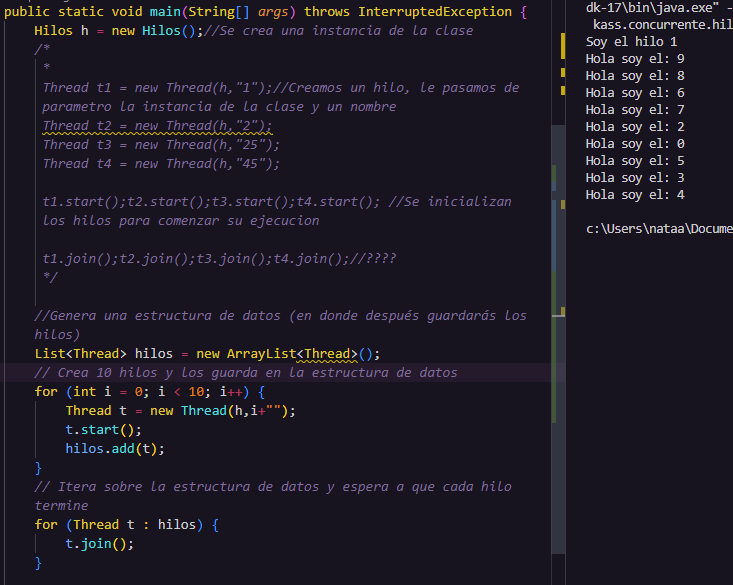
\includegraphics[width=\textwidth]{intro1.png}
        \caption{Hilos.java}
    \end{figure}
\end{enumerate}

\newpage
\section{Cuestionario}

\begin{enumerate}
    \item ¿Porque se utiliza Interrupted Exception en el método main?
    
    Es necesario indicar si un método puede lanzar una excepción, en este caso, el método main puede lanzar una excepción de tipo InterruptedException, la cual es lanzada cuando un hilo está esperando, durmiendo, u ocupado de alguna otra manera, y el hilo es interrumpido, ya sea antes o durante la actividad. 

    \item ¿Para que sirve el método Join?
    
    Espera a que este hilo muera. El método join permite que un hilo se una al final de otro hilo, es decir, detiene su ejecución hasta que el otro hilo termine.
    Supongamos que un hilo B no puede terminar su ejecución hasta que el hilo A haya terminado su tarea; entonces B se debe unir (join) a A y, por tanto, B no se va a ejecutar hasta que A termine.
    
    \item ¿Qué pasa si no le hacemos Join a los hilos?
    
    Si no se realiza un `join` a un hilo (o thread), el hilo se convierte en un "hilo detenido" cuando termina su ejecución. Esto significa que, aunque el hilo ha terminado de ejecutar su tarea, todavía mantiene algunos de sus recursos del sistema, como su identificador de hilo, hasta que se realiza un `join` en él. Si no se realiza un `join` en un hilo y se crean muchos hilos que terminan, estos hilos detenidos pueden consumir recursos del sistema y eventualmente llevar a la falta de recursos, como la incapacidad de crear nuevos hilos o procesos.

    \item ¿Cuáles son las ventajas de implementar Runnable contra extender de Thread?
    
    Runnable es una interfaz que es usada
    La interfaz Runnable debe ser implementada por cualquier clase cuyas instancias estén destinadas a ser ejecutadas por un hilo. La clase debe definir un método sin argumentos llamado run.
    
    Una clase que implemente Runnable puede ejecutarse sin subclasificar Thread instanciando una instancia de Thread y pasándose a sí misma como objetivo. En la mayoría de los casos, la interfaz Runnable se debe utilizar si sólo se planea sobrescribir el método run() y ningún otro método de Thread. Esto es importante porque las clases no deben ser subclasificadas a menos que el programador tenga la intención de modificar o mejorar el comportamiento fundamental de la clase.

    Un Thread es una cadena de ejecución en un programa. La máquina virtual Java permite que una aplicación tenga varios hilos de ejecución ejecutándose simultáneamente. Cada hilo tiene una prioridad, donde los hilos con mayor prioridad se ejecutan con preferencia a los hilos con menor prioridad. 
    
    \item ¿Cuál es la diferencia de implementar Runnable contra Callable?
    
    La interfaz Runnable debe ser implementada por cualquier clase cuyas instancias estén destinadas a ser ejecutadas por un hilo. La clase debe definir un método sin argumentos llamado run. Esta interfaz está diseñada para proporcionar un protocolo común para los objetos que desean ejecutar código mientras están activos

    La interfaz Callable es similar a Runnable, en el sentido de que ambas están diseñadas para clases cuyas instancias son potencialmente ejecutadas por otro hilo. Un Runnable, sin embargo, no devuelve un resultado y no puede lanzar una excepción verificada.

    \item ¿Se puede predecir el orden en el que se imprime el mensaje de la clase Hilos?
    
    No, por que el orden en el que se ejecutan los hilos es determinado por el sistema operativo.
    
    \item En el archivo Hilos2.java, ¿Qué pasa si sacamos la instancia de la clase “h” de t1, es decir, poner h antes de declarar t1?
    
    Si se saca la instancia de la clase "h" de t1, es decir, poner h antes de declarar t1, se obtendrá un error de compilación, ya que la variable h no está definida en el contexto de la clase Hilos.
    
    Si se se elimina tambien de la creación del thread t1, es decir  \texttt{Thread t1 = new Thread("1");}, ya no tendremos un error de compilación. 
    Pero al ejecutar el programa no tendremos salida en consola dado que el método run() no fue sobreescrito en la clase Hilos2, como era esperando al no haber un método run() sobreescrito, el método run() de la clase Thread es el que se ejecuta, el cual no tiene ninguna instrucción para imprimir en consola.

    \item Escribe que variables son locales (variables que estan en memoria del hilo) y que variables son compartidas de cada archivo y el por qué. Puedes tomarle captura al código y encerrar en un recuadro dichas variables.      
    
    Las variables locales son las que se encuentran dentro de un método run(), por ejemplo, las variables \texttt{a = 10} y \texttt{int b = 12}, cada hilo tiene su propia copia y eso lo podemos observar en la salida del programa, ya que cada hilo imprime su propio valor de a y b:
    
    \begin{figure}[h!]
        \centering
        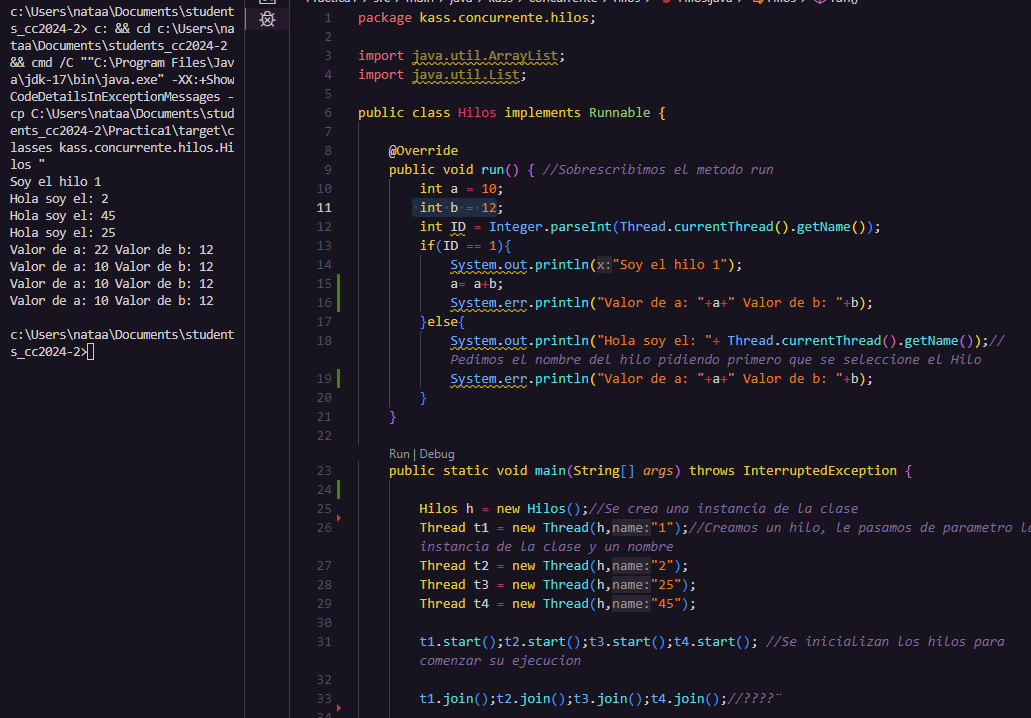
\includegraphics[width=\textwidth]{variablesLocales.png}
        \caption{Variables locales}
    \end{figure}

    
    \item \textbf{Contesta las preguntas de la sección de Synchronized}
    \item ¿Cómo podriamos darle un comportamiento diferente a los hilos?
    
\end{enumerate}

\section{Comentarios}
Escribe lo aprendido sobre esta práctica, así como tus conclusiones. También comparte si tuviste dificultades y los descubrimientos o alguna cosa de interés.


\section{Referencias}
\begin{itemize}
    \item Class InterruptedException. Oracle.
    
    \url{https://docs.oracle.com/javase/8/docs/api/java/lang/InterruptedException.html}
    
    \item Class Thread. Oracle. \url{https://docs.oracle.com/javase/8/docs/api/java/lang/Thread.html#join--}
    
    \item Solano, J. A. (2020). Hilos. Unidades de Apoyo para el Aprendizaje. CUAIEED/Facultad de Ingeniería-UNAM.
    
    \url{https://uapa.cuaieed.unam.mx/sites/default/files/minisite/static/a0b71f94-7e8c-4cf5-9bfc-cb7aad468992/UAPA-hilos/index.html}

    \item Interface Runnable. Oracle. 
    
    \url{https://docs.oracle.com/javase/8/docs/api/java/lang/Runnable.html}
\end{itemize}
\end{document}
